\documentclass[12pt, a4paper, oneside]{article}
\usepackage{caption, hyperref, listings}
\usepackage{graphicx}
% \usepackage[hyphens]{url}
\lstdefinestyle{mystyle}{
    basicstyle=\ttfamily,
    breaklines=true,
    showstringspaces=false,
    commentstyle=\color{gray},
    keywordstyle=\color{blue},
    numberstyle=\tiny\color{gray},
    numbers=left,
    frame=single,
    rulecolor=\color{black},
    backgroundcolor=\color{lightgray},
    xleftmargin=15pt,
    xrightmargin=5pt,
    morestring=[b]",
    morecomment=[l]{//},
}

\title{\textbf{A RISC-V computer system design}\thanks{\textit{Latest version available at:} \url{https://github.com/dream-tentacle/digital-logic-paper}}}

\author{Xiong Juncheng}
\date{\today}
\linespread{1.5}


\renewcommand{\abstractname}{\Large\textbf{Abstract}}

\begin{document}
\maketitle

\setcounter{page}{0}
\maketitle
\thispagestyle{empty}

\begin{abstract}
    In this project, I designed a simple RISC-V computer system on FPGA. The FPAG board is Digilent Nexys A7-100T. The compter system is composed of: a CPU, a data memory, an instruction memory, a vga screen, a keyboard, and a PWM audio output. The CPU is a 5-stage pipeline processor, which can execute 32-bit RISC-V instructions. The system interface is a terminal, which can execute basic commands and run two software - Snake and Piano.

    \textbf{Keywords}: RISC-V, FPGA, 5-stage pipeline, computer system
\end{abstract}
\newpage

\tableofcontents
\newpage

\setcounter{page}{1}
\section{Introduction}
\subsection{Overall introduction}

In the realm of digital systems design, the creation of a fully functional computer system on a Field-Programmable Gate Array (FPGA) stands as a testament to the designer's knowledge of digital systems. This project centers around the development of a simple yet robust RISC-V computer system, implemented on the Digilent Nexys A7-100T FPGA board. At the heart of this project lies the CPU, which is a 5-stage pipeline processor that can execute 32-bit RISC-V instructions. The computer system designed for this project includes essential components such as a CPU, a data memory, an instruction memory, a VGA screen, a keyboard, and a PWM audio output. The user interacts with the system through a terminal, which supports several commands and can run two software - Snake and Piano.

This report is divided into two parts. The first segment delves into the hardware design, concentrating on the intricacies of the 5-stage pipeline CPU, memory management, and all other devices. The second part shifts focus to the software design, encompassing the implementation of the terminal, the engaging Snake game, and the musical pursuit in the form of the Piano game.

\subsection{FPGA}
The FPGA board for this project is Digilent Nexys A7-100T, a circuit design and implementation platform for classroom use. For more information, please refer to \url{https://digilent.com/reference/programmable-logic/nexys-a7/start}.

\subsection{RISC-V}
RISC-V is an open-source instruction set architecture (ISA) based on reduced instruction set computer (RISC) principles. It is a standard ISA designed to be simple, extensible, and easy to implement. In this project, I implemented a 32-bit RISC-V CPU, which can execute all 37 base instructions. For more information about RISC-V itself, please refer to \url{https://riscv.org/}.
\section{Hardware}

\subsection{5-stage pipeline CPU}

\subsection{Memory management}

The CPU uses byte addressing, and access all other devices through memory-mapped I/O. The memory address is 32 bits wide, and the first 12 bits are used to select the device. The address map is shown in Table \ref{tab:address-map}.
\begin{table}[h]
    \centering
    \begin{tabular}{|c|c|c|}
        \hline
        Address range           & Device             \\
        \hline
        0x00000000 - 0x000FFFFF & Instruction memory \\
        \hline
        0x00100000 - 0x001FFFFF & Data memory        \\
        \hline
        0x00200000 - 0x002FFFFF & VGA screen         \\
        \hline
        0x00300000, 0x00300004  & Keyboard           \\
        \hline
        0x00400000, 0x00400004  & LED                \\
        \hline
        0x00500000, 0x00500004  & timer              \\
        \hline
        0x00600000              & deprecated         \\
        \hline
        0x00700000              & deprecated         \\
        \hline
        0x00800000, 0x00800004  & PWM audio output   \\
        \hline
    \end{tabular}
    \captionof{table}{Address Map}
    \label{tab:address-map}
\end{table}

\subsection{Instruction and data memory}
The instruction and data memory are both implemented using block RAM (BRAM). The instruction memory is read-only, and the data memory is read-write. Both of them are 1MB in size. The instruction address must be aligned to 4 bytes, while the data address can be any byte address.
\subsection{VGA screen (Write-only)}
The resolution is 640x480, and the color depth is 12 bits. Because the system is totally based on a terminal and the games are using characters as the basic unit, the screen is divided into 80x30 characters of 8x16 pixels. This allows us only store 80x30 characters' ascii code.

To accelerate the screen access speed, the screen is implemented with an one-dimensional array instead of a two-dimensional array. Considering the line and column size, 11-7 bits of the address are used to represent the line number, and 6-0 bits are used to represent the column number($2^5=32,2^7=128$). The screen has a base address of 0x00200000, and is accessed with 0x00200000 + offset.
\subsection{Keyboard (Read-only)}
The input signals of the keyboard are PS2\_CLK and PS2\_DATA. With a keyboard signal processor, a byte of scan code can be generated when a key is pressed. The scan code is then stored in a circular buffer of 16 bytes. The buffer provides the CPU with a "new\_key" signal, which is high when the buffer is not empty. The CPU can read "new\_key" through the address 0x00300000. When the CPU reads the address 0x00300004, the buffer will pop a byte of scan code.

The driver of the keyboard is implemented in the software part. Basically, the driver is a finite state machine (Figure \ref{fig:image1}), which can be divided into three states: KEY\_DOWN, KEY\_UP, LONG\_KEY\_DOWN, and LONG\_KEY\_UP. The "LONG\_" prefix in states refers to the two-bytes scan code which mainly start with 0xE0. The break code of a key is 0xF0 succeeded by its make code, thus the KEY\_UP and LONG\_KEY\_UP states are used to detect the break code.

The driver is implemented with a C function, which has only one state change every time it is called. There are three global values, "key\_ready", "two\_byte\_code" and "key\_up", which are signals for applications and are set according to the state. When the state machine finds that it ends a key press, it sets "key\_ready" to 1, and returns (the lowest byte of) the scan code. Otherwise, it returns 0.

The other two-byte scan codes are not used in this project, so we just ignore them.

\begin{figure}[!htb]
    \centering
    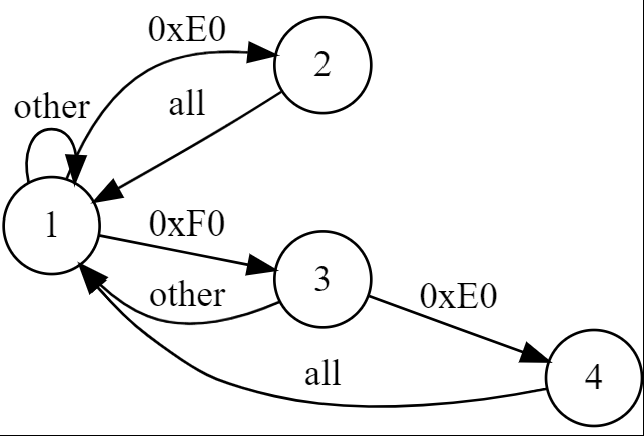
\includegraphics[width=8cm]{image1.png}
    \captionof{figure}{Keyboard driver state machine}
    \par 1: KEY\_DOWN, 2: LONG\_KEY\_DOWN, \\ 3: KEY\_UP, 4: LONG\_KEY\_UP
    \label{fig:image1}

\end{figure}


\subsection{PWM audio output (Write-only)}
The audio pitch is based on the frequency of the PWM signal. There is a count value and a max value. Thw PWM signal is high when the count value is less than half of the max value, and low otherwise. The count value is increased by 1 every clock cycle and set back to 0 when it exceeds the max value. Thus, the pitch can be adjusted by changing the max value.

The audio has two memory addresses, 0x00800000 and 0x00800004. The first address is used to set the max value, and the second address is used to turn on/off the audio.

\subsection{Timer (Read-only)}
There are two memory addresses, 0x00500000 and 0x00500004, corresponding to the millisecond counter and the second counter. Two extra counters are used for the timer. The first is a clock cycle counter that is set back to 0 when it exceeds $10^5$, and then both the second counter and the millisecond counter add 1. The second counter is set back to 0 when it exceeds 1000, and then the second counter adds 1. This implementation of four counters can largely reduce the complexity of the calculation because it doesn't use any division or multiplication.

\section{Software}
\subsection{Terminal}
The terminal is the interface between the user and the system. The function of the terminal calls the keyboard driver function only once every time it is called. If the keyboard driver returns 0, the terminal will return immediately. Otherwise, the terminal will process the scan code and execute the corresponding command. When the system is turned on, it enters a while loop, which calls the terminal function without stopping.

The terminal has different types of responses to different key presses:
\begin{itemize}
    \item \textbf{key up}: When the global variable "key\_up" is set to 1, the terminal checks if the key is "shift", "ctrl", or "alt". If so, it sets the corresponding global flag variable to 0. Otherwise, it does nothing.
    \item \textbf{key down}: When the global variable "key\_up" is set to 0:
          \begin{itemize}
              \item \textbf{signal keys}: If the key is "shift", "ctrl", or "alt", the terminal sets the corresponding global flag variable to 1.
              \item \textbf{backspace}: If the key is "backspace", the terminal deletes the last character in the buffer and put a space in the screen.
              \item \textbf{enter}: If the key is "enter", the terminal executes the command in the buffer. If the command is not recognized, the terminal does nothing.
              \item \textbf{caps lock}: If the key is "caps lock", the terminal toggles the "caps\_lock" global flag variable.
          \end{itemize}
\end{itemize}
The terminal supports the following commands:
\begin{itemize}
    \item \textbf{help}: Print the help message.
    \item \textbf{clear}: Clear the screen.
    \item \textbf{fib n}: Print the first n Fibonacci numbers.
    \item \textbf{sort n ...}: Sort the following n numbers.
    \item \textbf{prime n}: Print all prime numbers less than n (using Euler's sieve).
    \item \textbf{snake}: Run the Snake game.
    \item \textbf{piano}: Run the Piano game.
\end{itemize}
\subsection{Snake}

\subsection{Piano}

\end{document}